\label{chapt:intro}

It is hard to imagine there was ever a period of time where the need for instant communcation was a daily need. Constant access to cellular service and other telecommunication, regardless of location is something is not longer an option but a need. Up nearly 13\% from last year, it is said that US consumers are checking their mobile devices at a remarkable rate of 9 billion times per day \cite{deloittestat}.\\

It is numbers like these that have inspired \Company to begin research and development on a new way to provide this service more effectively. Altaeros is determined to develop the worlds first fully autonomous commercial aerostat's as a replacement to the conventional cellular tower. The latest version of their aerostat is seen below in Figure~\ref{fig:1_companypic}.

\begin{figure}[H]
	\centering
	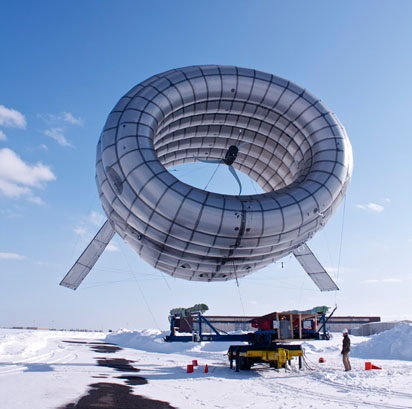
\includegraphics[scale=0.5]{1_companypic}
	\caption[Overview of Altaeros' aerostat.]{Overview of Altaeros' aerostat.\protect\cite{companypicweb}}
	\label{fig:1_companypic}
\end{figure}

From the above figure, the grounded tether management system can be observed. This report will focus one of the system's component structural design.

\section{Background} 

A key component responsible for full control of the aerostat is winch system. An overview of similar system used by Altaeros is shown below in Figure~\ref{fig:1_winch}.
\begin{figure}[H]
	\centering
	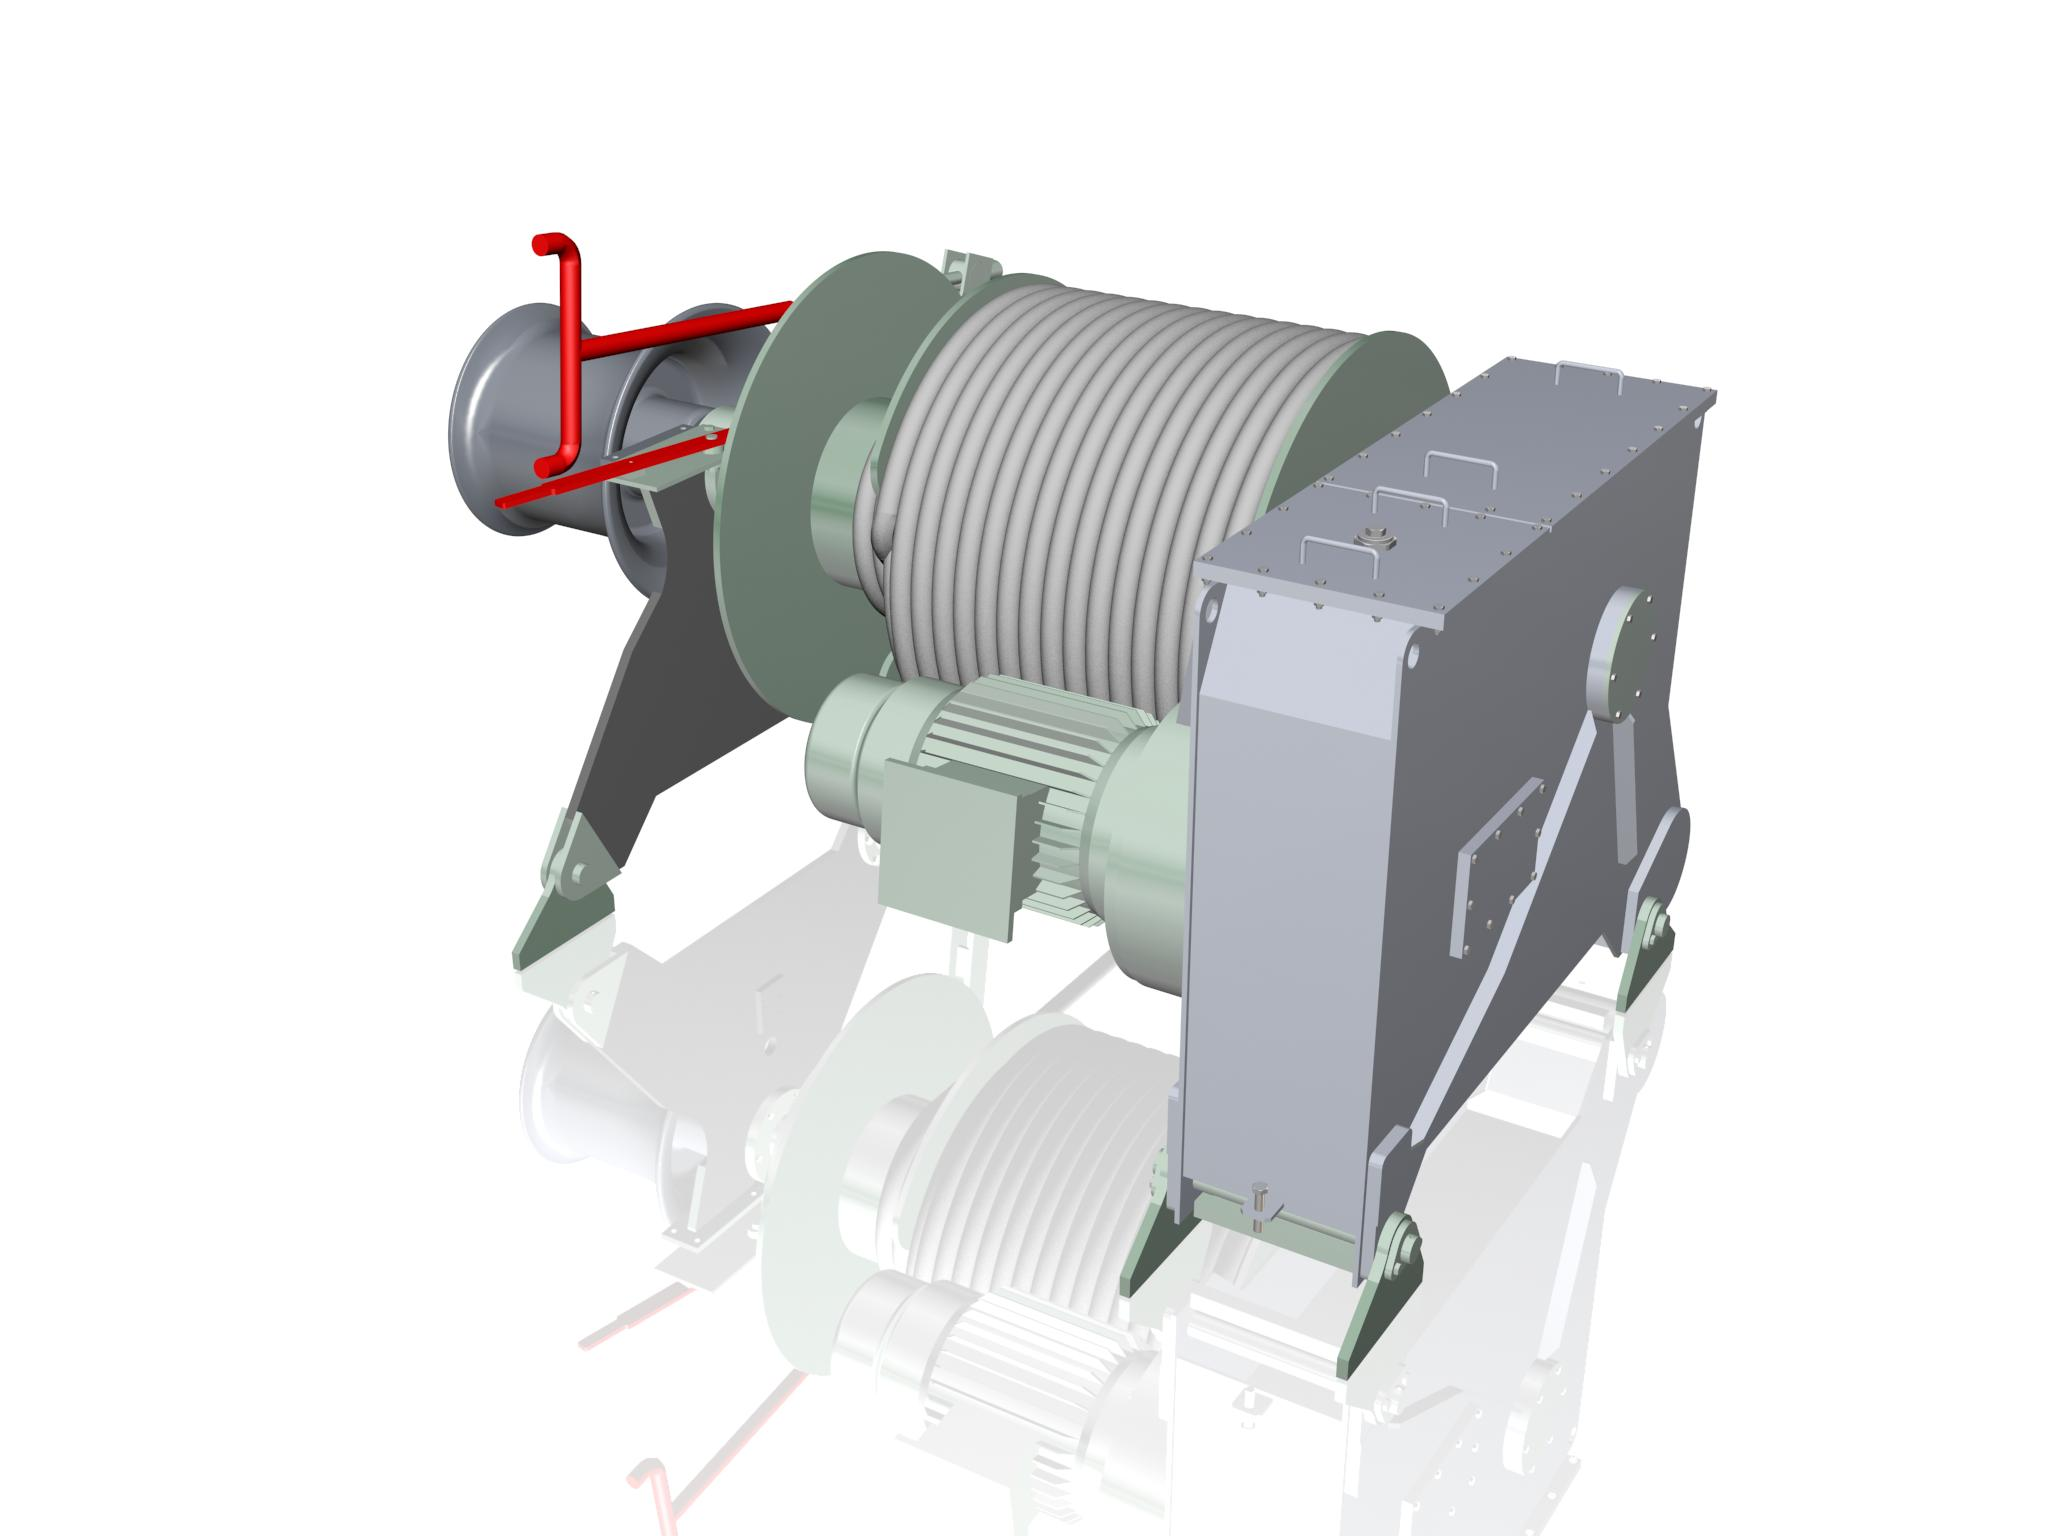
\includegraphics[scale=0.2]{1_winch}
	\caption[Example of common winch system.]{Example of common winch system.\protect\cite{winchpic}}
	\label{fig:1_winch}
\end{figure}

In the past, these winch systems were simply purchased by a third party vendor. After much though, it was deemed feasible that Altaeros could manufacture a more custom, cheaper and efficient winch system. In order to assure that the system is capable of handling the large aerodynamic loads translated by the tether, a complete structural analysis must be completed.

\section{Purpose}

The purpose of this report is to perform the structural analysis in order to assure that the winch drum assembly is capable of handling the large loads.\\

An overview of the winches drum assembly is shown from the 3D computer aided design (CAD) model developed with Inventor \cite{INVENTOR} as per Figure~\ref{fig:1_drum}.
\begin{figure}[H]
	\centering
	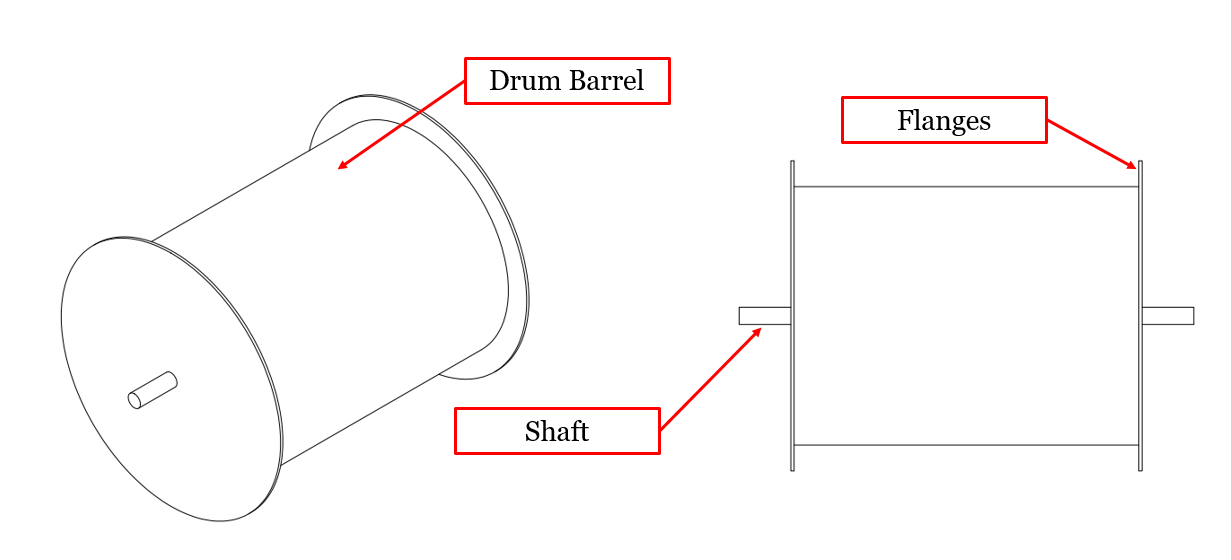
\includegraphics[scale=0.5]{1_drum}
	\caption{Drum assembly CAD model.}
	\label{fig:1_drum}
\end{figure}

It is important to realize that most of loading from the tether will be translated as pressure onto the barrel. This loading scenario will be investigated to properly size the winch barrel thicknesses which is the driving design dimension.

\section{Scope}

In the following sections of this report, the relevant parameters will be presented. From this, existing codes and standards will be investigated in exploring what a quick analysis would yield. From this, a more advanced numerical approach will be presented. These results will then be validated by use of finite element analysis (FEA). Finally, all results will be discussed, relevant conclusions and recommendations will be made.